\documentclass[a4paper]{article}
\usepackage[a4paper,left=3cm,right=2cm,top=2.5cm,bottom=2.5cm]{geometry}
\usepackage[utf8]{inputenc}
\usepackage{amsmath}
\usepackage{algorithm}
\floatname{algorithm}{Algorisme} % Cambia "Algorithm" por "Algorisme"

\usepackage{algpseudocode}
\usepackage{hyperref}
\usepackage{graphicx}
\usepackage{float}
\usepackage{array}

\title{\textbf{Intel·ligència Artificial:\\
		Pràctica SBC}}
\author{\emph{Guillem Cabré, Carla Cordero, Hannah Röber}}
\date{Curs 2024-25, Quadrimestre de tardor}

\renewcommand*\contentsname{Continguts}
\renewcommand{\figurename}{Figura}
\renewcommand{\tablename}{Taula}

\begin{document}
	
	\begin{titlepage}
		\clearpage\maketitle
		\thispagestyle{empty}
	\end{titlepage}
	
	\tableofcontents
	\clearpage
	
	\section{Identificació}
	
	\subsection{Descripció del problema}
	
	Els museus d’art són una de les principals atraccions turístiques a moltes ciutats, oferint l’oportunitat de gaudir d’obres mestres de diverses èpoques i estils. En el món real, els museus poden ser gegantescos, com per exemple el Museu del Louvre a Paris, el Museu Britànic a Londres, o el Museu del Prado a Madrid. Un dels problemes principals en visitar un museu és la limitació de temps per veure tot el que s’ofereix. Això genera la necessitat de desenvolupar aplicacions que ajudin els visitants a organitzar la seva visita de manera personalitzada. \\
	
	Els museus solen estar dividits en sales organitzades per artistes o per temes. Les obres d’art poden ser seleccionades en funció de diverses característiques, com l’any de creació, l’època, l’estil, l’autor, la sala on es troben, la temàtica, les dimensions, la complexitat o la importància de l’obra. A més, s’han de considerar els tipus de visitants i les seves preferències, com ara el temps disponible, el tipus de grup (individual, família, grup petit o gran) i el nivell de coneixement d’art. \\
	
	L’objectiu és crear una eina capaç d’ajustar la visita segons les preferències i característiques dels visitants, tenint en compte restriccions com el temps diari disponible i l’organització lògica de les sales.
	
	\subsection{Viabilitat del SBC}
	
	Abans de res, cal analitzar si el problema pot ser gestionat de manera òptima per un Sistema Basat en el Coneixement (SBC). Per plantejar-ho, ens fem la següent pregunta: seria possible que una persona experta en art dissenyés rutes personalitzades per a cada perfil de visitant d’un museu? La resposta és clara: sí. De fet, aquest ha estat el mètode tradicional, on les visites guiades han estat dissenyades per persones expertes en art. El nostre objectiu és modularitzar i automatitzar aquest procés, emulant el raonament d’un expert per dissenyar rutes òptimes entre les obres d’art d’un museu. \\
	
	A partir del problema plantejat, és evident que podem abstraure coneixement utilitzant una ontologia. Aquesta ontologia ens permetrà representar i relacionar els diferents conceptes clau del domini, com ara les característiques de les obres d’art, les preferències dels visitants i l’organització espacial del museu. A més, mitjançant l’ús de regles basades en aquest coneixement, podrem traçar un camí que ens guiï des del plantejament del problema fins a la seva solució de manera efectiva. \\
	
	Podem concloure que aquest enfocament ens permetrà construir un sistema capaç d’assistir els visitants de manera personalitzada i eficient.
	
	\subsection{Fonts del Coneixement}
	
	Tot el coneixement que integrarà el programa estarà organitzat en tres blocs principals:  
	\begin{itemize}  
		\item \textbf{Ontologia}: Aquest bloc ens permetrà relacionar els diferents conceptes de manera estructurada i organitzada. A més, serà fonamental per definir els atributs i les relacions entre aquests conceptes, oferint una base sòlida per al raonament del sistema.  
		
		\item \textbf{Instàncies}: Mitjançant CLIPS, es representarà tot aquell coneixement estàtic que es mantindrà invariable per a tots els visitants. Aquestes instàncies inclouran elements com les sales del museu, les obres d'art, els artistes, els estils pictòrics i fins i tot rutes predefinides del museu. Les rutes predefinides es descriuen amb més detall en una secció posterior.  
		
		\item \textbf{Visitant}: Per personalitzar l’experiència, el sistema recollirà informació sobre el visitant mitjançant un breu qüestionari. Aquest permetrà identificar les seves característiques i preferències, facilitant així la generació d’una ruta personalitzada que s’ajusti al màxim a les seves necessitats i interessos.  
	\end{itemize}
	
	\subsection{Objectius}
	
	Els objectius d’aquest projecte són:
	\begin{enumerate}
		\item Analitzar i modelar el domini dels museus per construir una ontologia adequada.
		\item Desenvolupar un sistema basat en coneixement capaç de proposar rutes de visita personalitzades.
		\item Implementar una solució en CLIPS que permeti simular visites segons les preferències i el temps disponible.
		\item Avaluar la solució mitjançant casos de prova representatius que validin la qualitat de les rutes generades.
	\end{enumerate}
	
	\subsection{Resultats Esperats}
	
	En finalitzar aquest projecte, s’espera obtenir els següents resultats:
	
	\begin{itemize}
		\item \textbf{Sistema Basat en Coneixement (SBC) operatiu}: Un sistema capaç de generar rutes personalitzades per als visitants del museu, tenint en compte les seves preferències i el temps disponible.
		
		\item \textbf{Ontologia del domini dels museus}: Una representació formal dels conceptes i les relacions del domini, que permeti al sistema raonar de manera eficient.
		
		\item \textbf{Generació automàtica de rutes personalitzades}: Un procés automatitzat que utilitzi les preferències del visitant per crear una ruta òptima que maximitzi l'experiència de la visita.
		
		\item \textbf{Avaluació mitjançant casos de prova}: La validació del sistema es durà a terme mitjançant proves representatives que permetin avaluar l'eficàcia i l'eficiència de les rutes generades.
	\end{itemize}
	
	Tot i que aquest projecte ha estat dissenyat com a part d'una tasca universitària, l'objectiu principal és aprendre a implementar Sistemes Basats en Coneixement (SBC). Encara que el projecte no es lliurarà a cap museu perquè en faci ús, ens agradaria que servís com a fonament per a futurs projectes viables en la vida real, amb l'objectiu de personalitzar rutes de visita en museus.
	
	\newpage
	\section{Conceptualització}
	
	La conceptualització d'aquest projecte es basa en la identificació, definició i descripció dels elements fonamentals que conformen el domini. Aquesta etapa és clau, ja que permet establir les bases conceptuals necessàries per al desenvolupament del sistema, garantint així una implementació coherent amb els objectius inicials. \\
	
	Les relacions entre aquests elements és fonamental, ja que el sistema ha de ser capaç de generar recomanacions personalitzades de rutes de visita tenint en compte les preferències dels visitants, les característiques de les obres d'art i la distribució de les sales. Per assolir aquest objectiu, s'han definit atributs específics per cada element que permeten emmagatzemar dades rellevants, com la complexitat d'una obra, la durada disponible de la visita o la preferència per certs estils artístics. Aquesta informació es recull de forma automàtica a través d'un conjunt de preguntes inicials, que pretenen conèixer el perfil del visitant i els seus interessos. \\
	
	Mitjançant la definició clara i precisa dels conceptes del domini, es redueixen les possibles ambigüitats del disseny i es faciliten els mecanismes de personalització de les rutes. \\
		
	\subsection{Elements del domini}
	\label{sec:elements_del_domini}
	
	Els elements del domini fonamenten el SBC. Cada element té una funció específica i es defineix mitjançant atributs que en descriuen les seves propietats rellevants. Aquesta classificació permet organitzar la informació de forma estructurada i facilitar les relacions entre ells. \\
	
	\noindent \textbf{Característiques d'una visita}
	\begin{itemize}
		\item \texttt{Definició}: Representen les persones que fan una visita al museu.
		\item \texttt{Atributs}:
		\begin{itemize}
			\item \texttt{Nombre persones}: Número de persones que formen el grup de visita. Pot ser individual (una persona), o un grup.
			\item \texttt{Nombre museus visitats}: Nombre de museos visitats l'últim any, d'aquí derivará el càlcul de coneixement de la visita sobre museus.
			\item \texttt{Durada diària}: Temps disponible per dia (hores).
			\item \texttt{Dies totals}: Nombre de dies disponibles per a la visita.
			\item \texttt{Familia}: Hi ha nens al grup.
			\item \texttt{Preferència d'artista}: Artista d'interès per la visita.
			\item \texttt{Preferència d'estil}: Estil d'interès per la visita.
		\end{itemize}
	\end{itemize}
		
		
	\noindent \textbf{Característiques d'un autor}
	\begin{itemize}
		\item \texttt{Definició}: Artistes creadors de les obres del museu.
		\item \texttt{Atributs}:
		\begin{itemize}
			\item \texttt{Nom}: Identificació de l’artista.
			\item \texttt{Nacionalitat}
			\item \texttt{Estil}: Interval històric de temps en què va crear obres.
			
		\end{itemize}
	\end{itemize}
	
	
	\noindent \textbf{Característiques d'una obra d'art}
	\begin{itemize}
		\item \texttt{Definició}: Objecte del museu amb unes certes característiques.
		\item \texttt{Atributs}:
			\begin{itemize}
				\item \texttt{Títol}: Nom de l’obra (p. ex., "La Gioconda").
				\item \texttt{Autor}: Referència a l’autor que ha creat l'obra.
				\item \texttt{Any de creació}
				\item \texttt{Estil}: Període històric en què es va crear (p. ex., Renaixement).
				\item \texttt{Sala}: Ubicació al museu.
				\item \texttt{Dimensions}
				\item \texttt{Complexitat}: Calculada a partir de les mides de l'obra.
			\end{itemize}
	\end{itemize}


	\noindent \textbf{Característiques d'una sala d'art}
	\begin{itemize}
		\item \texttt{Definició}: Espai on s'exposen un conjunt d'obres d'art.
		\item \texttt{Atributs}:
		\begin{itemize}
			\item \texttt{Museu al que pertany}
		\end{itemize}
		\item \texttt{Subclasses}:
		\begin{itemize}
			\item \texttt{Sala Artista}: Sala dedicada a exposar les obres d'un artista concret.
			\item \texttt{Sala Estil}: Sala dedicada a exposar les obres d'un estil concret.
		\end{itemize}
	\end{itemize}
	
	\subsubsection{Selecció d'obres}
	
	Tot i que aquest projecte no representa un museu real, tampoc la seva representació al sistema ho serà. Aquesta decisió es va prendre pel fet que la complexitat de seleccionar un gran nombre d'obres d'un museu, com el Prado o el Louvre, era massa elevada, especialment considerant que no estem davant d'un problema de la vida real. Si haguéssim considerat necessari utilitzar un conjunt més ampli d'obres, hauríem pogut implementar un \textit{scraper} en \textit{Python} per obtenir un fitxer amb totes les instàncies necessàries i inserir-les a l'ontologia. No obstant això, vam decidir optar per una solució més senzilla que s'ajustés millor als objectius del projecte.\\
	
	El nostre museu estarà compost per un nombre limitat d'estils artístics. Concretament, hem seleccionat tres estils principals: Barroc, Contemporani i Renaixentista. Tant les obres com els autors que s'exposaran al museu pertanyen a aquests estils. Com que cap membre del grup és expert en art, vam optar per fer ús d'una eina externa per facilitar la selecció. Concretament, vam utilitzar \textit{ChatGPT} per obtenir una llista de 5 artistes rellevants de cada període i, per a cadascun d'ells, una selecció de 5 de les seves obres més representatives.\\
	
	Un cop rebuda la llista suggerida, la vam revisar per identificar possibles errors i adaptar-la a les nostres necessitats. Com a resultat, vam obtenir una configuració final composta per $3$ estils, $15$ autors ($3 \times 5$) i $75$ obres ($3 \times 5 \times 5$). Aquesta selecció ens permet treballar amb un conjunt de dades manejable però suficientment representatiu per als nostres objectius de prova i validació del sistema.
	
	\subsection{Divisió en subproblemes}
	\label{sec:Subproblemes}
	
	\subsubsection{Problema concret: Recollir dades de la visita}
	
	Abans de començar a buscar una solució pel problema, és necessari recopilar la informació rellevant sobre el perfil dels visitants. Aquesta informació es recull mitjançant un conjunt de preguntes que permeten identificar:
	\begin{itemize}
		\item Les característiques generals del grup: tipus (individual, família, grup petit o grup gran) i coneixement d’art (baix, mitjà o alt).
		\item Les limitacions temporals de la visita, incloent-hi el nombre de dies disponibles i la durada màxima per jornada.
		\item Les preferències personals dels visitants, com ara estils artístics i autors favorits.
	\end{itemize}
	
	Aquestes dades són essencials per personalitzar l’experiència del visitant i garantir que el pla de visita s’ajusti als seus interessos i necessitats.
	
	\paragraph{Preguntes inicials per al visitant:}
	A continuació, es presenta el conjunt de preguntes que es fan als visitants per tal de recollir aquesta informació:
	\begin{itemize}
		\item \textbf{Sobre el grup:}
		\begin{itemize}
			\item Quantes persones sou? 
			\begin{itemize}
				\item Resposta numèrica
			\end{itemize}
			\item Hi ha nens al grup? 
			\begin{itemize}
				\item Sí
				\item No
			\end{itemize}
			\item Quants museus heu visitat l'últim any? 
			\begin{itemize}
				\item Resposta numèrica
			\end{itemize}
		\end{itemize}
		
		\item \textbf{Sobre el temps de visita:}
		\begin{itemize}
			\item Quants dies teniu disponibles per visitar el museu?
			\item Quantes hores podeu dedicar-hi cada dia?
		\end{itemize}
		
		\item \textbf{Sobre les preferències:}
		\begin{itemize}
			\item Hi ha algun estil/època artística que us interessi especialment?
			\item Hi ha algun autor que us agradaria veure?
		\end{itemize}
		Per aquestes preguntes es mostra el conjunt d'opcions disponible al museu, també una opció per si no es vol marcar preferència.
	\end{itemize}

	
	\subsubsection{Abstracció: analitzar els interessos de la visita}
	
	Un cop recollides les dades, es crea el problema abstracte. El sistema analitza les preferències i característiques proporcionades pels visitants. Aquesta anàlisi inclou:
	\begin{itemize}
		\item Determinar si la visita serà curta o llarga en funció de les hores i dies que l'usuari ha indicat.
		\item Guardar si la visita serà individual, o d'un grup gran o petit, en funció del nombre de persones que la formen.
		\item Determinar el grau de coneixement en art de la visita.
		\item Emmagatzemar les preferències d'estil de la visita.
	\end{itemize}
	
	El resultat d’aquest procés és el problema abstracte i servirà com a base per planificar la visita.
	
	
	\subsubsection{Associació: Generar una solució abstracte}

	Partint del problema abstracte, el sistema s’encarrega de trobar un conjunt d'obres d'art tenint en compte les necessitats trobades. Això inclou:
	\begin{itemize}
		\item Seleccionar un conjunt d'obres seguint els interessos dels visitants.
		\item Determinar un conjunt d'obres tenint en compte el temps de la visita i estimant el temps necessari per observar cada obra.
		\item Assignar un ordre lògic a les obres seleccionades, minimitzant els salts innecessaris entre sales.
	\end{itemize}
	
	L’objectiu és proporcionar un recorregut coherent i fàcil de seguir que maximitzi l’aprofitament del temps dels visitants.
	
	\subsubsection{Refinament: Creació d'una solució concreta}
	
	Adaptem el recorregut, assegurant que la durada total de cada jornada no superi les hores disponibles. Finalment, el sistema genera una proposta completa i personalitzada per al visitant, amb una llista d'obres agrupades per sales. \\
	
	El procés d'adaptació del recorregut seleccionat a les preferències del visitant serà el següent:
	\begin{itemize}
		\item Afegir totes les obres de l'autor preferit pel visitant, si aquest té una preferència específica.
		\item Afegir totes les obres de l'estil pictòric preferit del visitant, si en té.
		\item Ajustar el temps de la següent manera: 
		\begin{itemize}
			\item Si el temps estimat de la ruta és superior al temps que el visitant vol destinar, eliminarem obres segons el seu grau de complexitat i el coneixement del visitant. Si el visitant té un coneixement elevat, es treuran les obres menys complexes; i a l'inrevés, si el coneixement és baix, es retiraran les obres més complexes.
			\item Si el temps estimat de la ruta és inferior al temps disponible, afegirem obres seguint la mateixa regla que anteriorment. Si el visitant és expert en art, afegirem obres amb una complexitat elevada. I si no ho és, afegirem obres de complexitat reduïda.
		\end{itemize}
	\end{itemize}
	
	Un cop tenim la selecció final, es retornaran les obres ordenades per sales. D'aquesta manera, l'usuari podrà optimitzar el seu temps sense canviar de sala innecessàriament. \\
	
	Cal tenir en compte que, com a temps mitjà per obra, hem establert 15 minuts. En futures versions del sistema, seria interessant ajustar el temps dedicat a cada obra depenent de la seva complexitat i, a més, en funció de qui la visiti. No es triga el mateix a observar la Mona Lisa per part d'un nen petit que per part d'un expert en art, ja que aquest últim es fixarà en cada pinzellada.
	
	\subsection{Identificació de conceptes principals}
	
	\subsubsection{Tipus de visites}
	Les visites al museu es poden classificar segons diversos criteris relacionats amb el perfil dels visitants i les seves necessitats:
	\begin{itemize}
		\item \texttt{Tipus de grup}:
		\begin{itemize}
			\item Individual
			\item Grup petit (2-5 persones)
			\item Grup gran (més de 5 persones)
		\end{itemize}
		\item \texttt{Durada de la visita}:
		\begin{itemize}
			\item Curta: 5 hores o menys per tota la visita
			\item Llarga: més de 5 hores
		\end{itemize}
		\item \texttt{Coneixement artístic}:
		\begin{itemize}
			\item Baix: ha visitat pocs museus, per tant, suposem que coneix poques obres o autors.
			\item Mitjà: coneix algunes èpoques o estils.
			\item Alt: coneix moltes obres i autors, pot visitar obres més complexes
		\end{itemize}
	\end{itemize}
	
	\subsubsection{Disseny del museu}
	El museu tracta principalment sobre tres èpoques clau de la història de l'art: {Renaixement, Barroc i Art Modern}. De cadascuna d'aquestes èpoques comptem amb un gran ventall d'artistes que han estat representatius. És per això que aquest està organitzat en diferents sales que agrupen totes les obres artístiques segons criteris específics.
	
	Tenim sales dedicades a cadascuna d'aquestes èpoques. A més, també hi ha sales dedicades a alguns dels artistes més importants d'aquests grans moments històrics. Algunes de les sales disponibles són:
	
	\begin{itemize}
		\item \texttt{Sales Temàtiques: } 
		\begin{itemize}
			\item Renaixement
			\item Barroc
			\item Art Modern
		\end{itemize}
	\end{itemize}
	
	\begin{itemize}
		\item \texttt{Sales sobre artistes: } 
		\begin{itemize}
			\item Claude Monet: Artista d'Art Modern
			\item Wassily Kandinsky: Artista d'Art Modern
			\item ArtemisiaGentileschi: Artista del Barroc
			\item Rembrandt Van Rijn: Artista del Barroc
		\end{itemize}
	\end{itemize}
	
	\newpage
	\section{Formalització}
	
	\subsection{Desenvolupament de la ontologia}
	
	Per a resoldre el problema plantejat de recomanació de rutes en un museu utilitzant sistemes basats en el coneixement, hem desenvolupat una ontologia que descriu els elements que hem considerat clau d’aquest entorn i com es relacionen, com ara artistes, obres d’art, estil, sales, museus i visites. Inicialment, aquesta ontologia es va implementar en Protégé, una eina àmpliament utilitzada per a la creació d’ontologies en el llenguatge OWL (Web Ontology Language). Aquesta fase ens ha permès estructurar els conceptes i relacions de manera formal i estandarditzada. \\
	
	Posteriorment, hem convertit l’ontologia juntament amb les instàncies pertinents escollides a format CLIPS per poder integrar-la en un sistema basat en regles, que facilita la inferència automàtica de recomanacions. En aquest sistema, l’ontologia funciona com a base de coneixement, mentre que un conjunt de regles defineixen la lògica de recomanació per personalitzar les rutes en funció de les preferències dels visitants, les característiques de les sales i la disponibilitat d’obres. \\
	
	Aquest enfocament ens permet aprofitar els beneficis d’una representació formal del coneixement combinada amb la capacitat de raonament d’un sistema expert. A continuació, es descriuen les classes principals de l’ontologia, els seus atributs, les seves funcions dins del sistema i com es relacionen. Vegeu a continuació el diagrama de la ontologia: \\
	
	\begin{figure}[H]
		\centering
		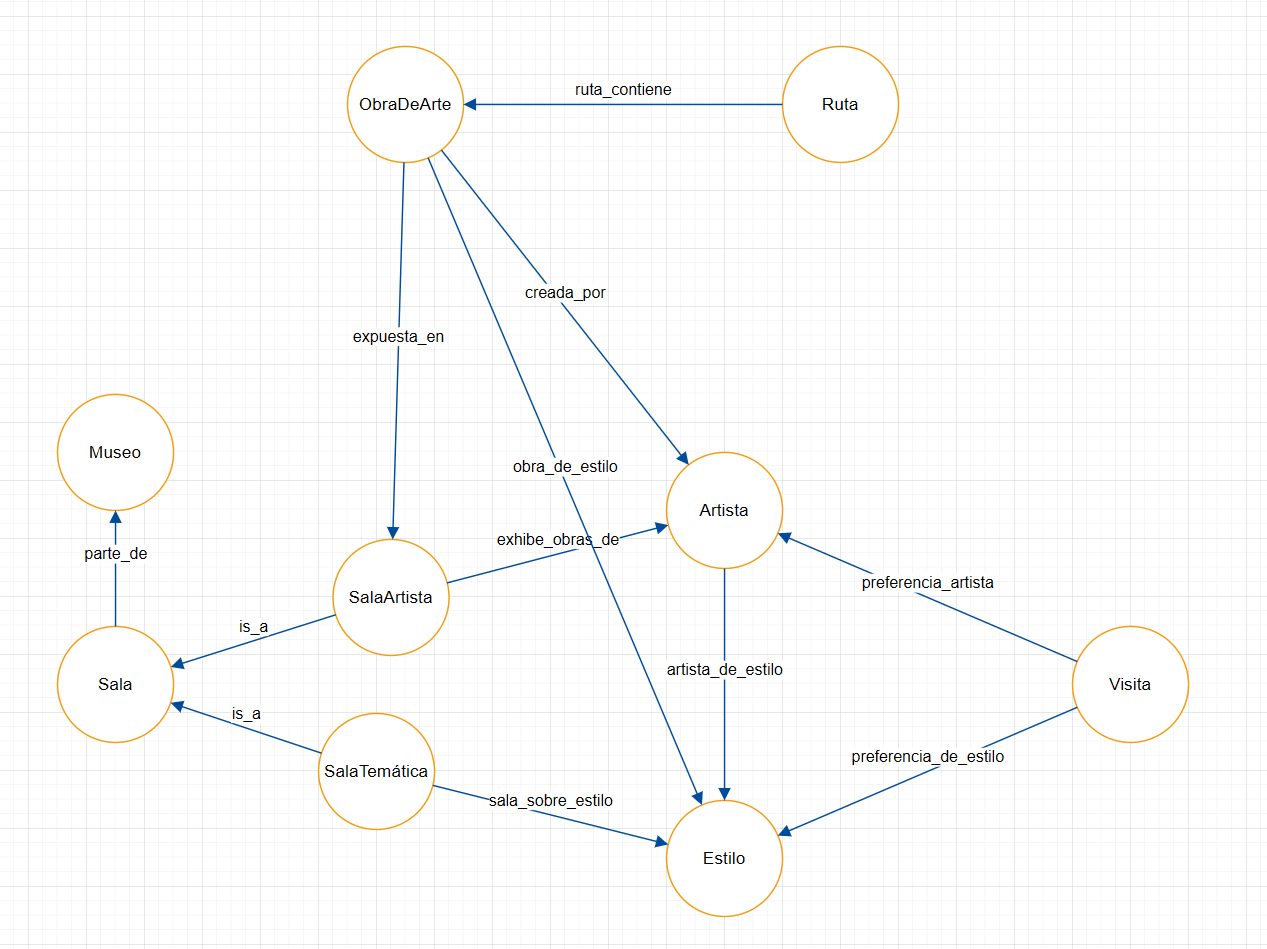
\includegraphics[width=0.75\linewidth]{images/ontologia.png}
		\caption{Diagrama de la ontologia del SBC}
	\end{figure}
	
	\subsubsection*{Artista}
	Representa el concepte d'artista dins del sistema, el creador de les obres d'art que estan exhibides al museu. Aquesta classe inclou informació rellevant sobre cada artista, com ara el seu nom i les seves obres destacades que té exposades al museu. Els artistes estan connectats amb les seves obres a través de relacions específiques i tenen associats estils d'art.
	
	Atributs de la classe:
	\begin{itemize}
		\item \texttt{artista\_de\_estilo}: Estils artístics associats a l’artista, amb els quals crea les obres.
	\end{itemize}
	
	
	\subsubsection*{Museu}
	És l'entitat central de l'ontologia i de tot el problema, que encapsula totes les altres classes. Un museu està conformat per una o múltiples Sales, cadascuna amb una funció específica (temàtica o basada en artistes). En cada sala hi ha exposades totes les diferents obres dels artistes que poseeix el museu per a que puguin ser admirades i observades pels visitants durant la seva visita al museu recorrent la ruta recomanada pel nostre sistema.
	
	\subsubsection*{Obra d'Art}
	Representa cada peça exhibida al museu, les quals seran observades durant el recorregut de la ruta pel museu dels visitants. Inclou atributs com el títol, l'artista associat que l'ha creada, l'any de creació. Les obres estan vinculades amb els artistes que les han creat, les sales on s'exhibeixen i l'estil amb el qual han estat elaborades.\\
	Atributs de la classe:
	\begin{itemize}
		\item \texttt{creada\_por}: Artista que va crear l’obra.
		\item \texttt{expuesta\_en}: Sala on es troba exposada.
		\item \texttt{obra\_de\_estilo}: Estil artístic de l’obra.
		\item \texttt{Dimensiones}: Dimensions físiques de l’obra.
		\item \texttt{añoCreacion}: Any en què es va crear l’obra.
	\end{itemize}
		
	\subsubsection*{Ruta}
	Defineix recorreguts optimitzats i predefinits ja per als visitants. Cada ruta pot estar basada en criteris com preferències artístiques, limitacions de temps, temàtiques d'interès o grau de coneixement en art. Per exemple, una ruta pot connectar les sales dedicades a un estil artístic o incloure només obres més complexes per als experts.\\
	Atributs de la classe:
	\begin{itemize}
		\item \texttt{ruta\_contiene}: Llista d'obres d'art incloses en la ruta per a que les puguin observar els visitants en ordre.
	\end{itemize}
	
	\subsubsection*{Sala}
	Representa els espais on estan exposades les obres dins del museu.
	Atributs de la classe:
	\begin{itemize}
		\item \texttt{parte\_de}: Indica el museu al qual pertany la sala.
	\end{itemize}
	 Aquesta classe té dues subclasses que són les següents:
	
	\begin{itemize}
		\item \textbf{SalaArtista}: Dedicada a un artista específic, on totes les obres exhibides són del mateix autor.\\
		Atributs de la subclasse:
			\begin{itemize}
				\item \texttt{exhibe\_obras\_de}: Artista al que està dedicat la sala i on totes les obres són seves.
			\end{itemize}
	\item \textbf{SalaTemàtica}: Sala amb un estil i amb obres d'una mateix estil artístic. Les sales poden tenir atributs com el nom i estar vinculades a un estil concret.\\
		Atributs de la subclasse:
		\begin{itemize}
			\item \texttt{sala\_sobre\_estilo}: Estil artístic de la sala i en conseqüència de les obres exhibides, les obres poden ser de diferents artistes.
		\end{itemize}
	\end{itemize}
		
	\subsubsection*{Visita}
	Representa una instància d'interacció d'un visitant o grup amb el museu. Aquesta classe emmagatzema les dades que caracteritzen a la entitat visita que ve a visitar el museu, i també les seves preferències, permetent així personalitzar l'experiència al màxim perquè puguin aprofitar la visita al museu en base a les dades recopilades. Els atributs (dades dels visitants) en minúscules s'extreuen a la part de recopilació mitjançant preguntes i els atributs en majúscules es deriven dels altres atributs.\\
	Atributs de la classe:
	\begin{itemize}
		\item \texttt{preferencia\_artista}: Preferències del visitant sobre algun artista del museu, si és que en té.
	 	\item \texttt{preferencia\_de\_estilo}: Estil preferit del visitant dels que hi ha al museu, si és que en té.
		\item \texttt{nHoras/Dia}: Nombre d’hores que el visitant pot dedicar al museu per dia.
		\item \texttt{CONOCIMIENTO}: Grau de coneixement sobre art del visitant.
		\item \texttt{DURACIÓN}: Durada total de la visita.
		\item \texttt{ESTILOPREFERIDO}: Estil artístic favorit del visitant.
		\item \texttt{TIPOGRUPO}: Tipus de grup i la seva mida, si es individual, petit o gran.
		\item \texttt{esFamilia}: Indica si la visita és d’un grup familiar i té nens si no es individual el grup.
		\item \texttt{nDias}: Nombre de dies dedicats a la visita.
		\item \texttt{nMuseosVisitados}: Nombre de museus visitats pel grup o individu durant l'últim any. Ens serveix per saber quant de coneixement en art té el grup.
	 	\item \texttt{nPersonas}: Nombre total de persones al grup. Per determinar el tipus de grup.
	\end{itemize}

	
	\subsubsection*{Estil}
	Defineix els estils artístics representats al museu que poden definir una obra d'art, un artista o també una sala temàtica.\\
	Atributs de la classe:
	\begin{itemize}
		\item \texttt{tipo}: Tipus específic d’estil artístic. (barroc, renaixement, modernisme, etc.).
	\end{itemize}
	
	
	\subsection{Justificació de la metodologia de resolució}
	
	La metodologia utilitzada per resoldre el problema es basa en una divisió clara del sistema en diferents mòduls independents. Aquesta elecció es justifica per les següents raons:
	
	\begin{itemize}
		\item \texttt{Estructura modular:} El problema de generar rutes personalitzades per als visitants d’un museu es compon de diverses parts:
		\begin{itemize}
			\item Recopilació de dades dels visitants.
			\item Abstracció i classificació de la visita.
			\item Associació d’obres i sales en funció de les preferències i limitacions.
			\item Refinament i optimització final de les rutes.
		\end{itemize}
		Aquesta divisió permet abordar cada part de forma independent, reduint la complexitat del desenvolupament i assegurant que cada component funcioni correctament abans d’integrar-lo al sistema complet.
		
		\item \texttt{Flexibilitat i manteniment:} L'ús de mòduls clarament definits facilita la modificació i ampliació del sistema en el futur. Per exemple, es poden afegir nous estils d’art, obres o criteris de personalització sense afectar altres parts del sistema.
		
		\item \texttt{Evolució incremental:} El sistema construeix la solució de manera progressiva, començant per la recopilació de dades, seguint amb l’anàlisi i generació d’una ruta inicial, i acabant amb el refinament i l’optimització. Aquest enfocament escalonat garanteix que cada pas afegeixi un nivell de detall fins a obtenir una solució ajustada a les necessitats del visitant.
		
	\end{itemize}
	
	En conjunt, aquesta metodologia assegura que el sistema sigui escalable i fàcil de gestionar, de la mateixa forma que, en un futur, permet aplicar nous canvis en els criteris seleccionats.

	
	\newpage
	\section{Implementació}
	
	La implementació del sistema s'ha estructurat en diverses fases, cadascuna centrada en una part específica del desenvolupament. A continuació, es detallen les principals etapes i les tasques realitzades en cadascuna:
	
	\subsection{Creació de l’ontologia i instàncies}
	
	L’ontologia ha estat dissenyada per representar de forma estructurada els conceptes clau del domini: les classes i els atributs per modelar el museu. Un cop definida aquesta amb Protegé, incloent els elements del domini explicats en apartats anteriors, s'han creat les instàncies estàtiques del museu, buscant un conjunt representatiu de: sales obres d'art, artistes i èpoques.
	
	\subsection{MAIN}
	\begin{itemize}
		\item Mòdul principal que actua com a punt d’entrada.
		\item Activa la seqüència de preguntes per al visitant i inicialitza el flux d’execució del sistema.
	\end{itemize}
	
	
	\subsection{Mòdul "recopilacion": recopilació de dades}
	
	Aquest mòdul inclou regles i funcions encarregades d'obtenir informació inicial dels visitants a través de preguntes interactives. Les dades recollides inclouen:
	\begin{itemize}
		\item Característiques del grup: Nombre de persones, presència de nens i experiència prèvia (nombre de museus visitats).
		\item Duració de la visita: Dies disponibles i hores per dia.
		\item Preferències: Estils artístics i artistes favorits.
	\end{itemize}
	Les respostes es processen i s'emmagatzemen com a fets per a l'ús posterior del sistema.
	
	
	\subsection{Mòdul "abstraccion": d’abstracció}
	
	Un cop recollides les dades, aquest mòdul transforma la informació inicial en un problema abstracte. Les tasques realitzades inclouen:
	\begin{itemize}
		\item Classificació del grup: Individual, grup petit o grup gran.
		\item Determinació del coneixement artístic: Baix, mitjà o alt, basat en el nombre de museus visitats.
		\item Càlcul de la durada de la visita: Curta o llarga, segons els dies i hores disponibles.
	\end{itemize}
	Aquestes classificacions serveixen com a base per a la generació de rutes.
	
	\subsection{Mòdul de matching}
	
	Aquest mòdul genera una primera ruta pel visitant basada en les seves preferències i característiques, és a dir, en el seu interès en art i en el seu coneixement. \\
	
	Aquest mòdul prioritza les obres i sales més rellevants per al visitant.
	
	\subsection{Mòdul de refinament}
	
	Aquest mòdul ajusta la ruta inicial per adaptar-la millor a les necessitats del visitant:
	\begin{itemize}
		\item Afegir obres d'artistes i estils preferits no inclosos inicialment.
		\item Afegir o treure obres en funció del temps disponible i el seu coneixement.
	\end{itemize}
	El resultat és una ruta final personalitzada i agrupada de forma lògica.
	
	\subsection{Resultats generats}
	
	Un cop completats tots els passos, el sistema presenta al visitant una ruta final amb les obres seleccionades, ordenades per sales i sessions diàries. \\
	
	Aquest resultat intenta ajustar-se al perfil del visitant i maximitzar l’aprofitament del temps.
	
	
	\newpage
	\section{Jocs de Prova}
	
	Per validar la funcionalitat i robustesa del sistema de personalització de visites al museu, hem dissenyat sis jocs de prova que cobreixen diferents escenaris. Cada cas està pensat per posar a prova aspectes específics del sistema, tenint en compte variables com el tipus de visitant, el temps disponible, el coneixement sobre art i les preferències temàtiques. En aquest apartat es descriu cada prova detalladament, es justifica el seu objectiu i es presenta la sortida esperada de forma genèrica.
	
	\subsection{Prova 1: Visita Familiar amb Nens}
	
	\paragraph{Objectiu:} 
	Aquest joc de prova està dissenyat per avaluar si el sistema és capaç de recomanar una ruta adequada per a una família amb nens, prioritzant obres fàcils d’entendre i visuals. També es verifica que el sistema maximitzi l’ús del temps disponible sense sobrecarregar la visita.
	
	\paragraph{Descripció del cas:} 
	
	\begin{itemize}
		\item \textbf{Nombre de persones:} 5.
		\item \textbf{Hi ha nens?} Sí.
		\item \textbf{Hi ha més nens que adults?} Sí.
		\item \textbf{Durada de la visita:} 1 dia de 3 hores.
		\item \textbf{Coneixement d’art:} Baix (1 museu visitat).
		\item \textbf{Preferències:} Sense preferències específiques.
	\end{itemize}
	
	\paragraph{Sortida esperada:}
	El sistema hauria de seleccionar una ruta que inclogui obres i sales adequades per a nens, és a dir, obres simples, de poca compexitat. També s’hauria de garantir que les obres siguin variades (diferents èpoques) i que el recorregut proposat estigui ben ordenat per sales. A més, com és un grup petit i amb nens, i està pensat que es dediquin uns 10 minuts per obra en aquest cas, s'espera un recorregut d'unes 18 obres.
	
	\paragraph{Sortida obtinguda:}
	En general, els resultats són els esperats pel cas plantejat. Primer de tot, veiem que el nombre d'obres es correspon al que esperàvem: 18. Per altra banda, també veiem que les obres no són de gran complexitat i que la ruta està ben estructurada pel que fa al recorregut per sales \\
	
	Per últim, destacar que els estils són variats, com s'esperava tenint en compte que no havíem marcat cap preferència en concret, tot i que és cert que predominen més les obres del Renaixement.
	
	\subsection{Prova 2: Grup Gran d’Adults}
	
	\paragraph{Objectiu:} 
	Aquest joc de prova pretén verificar com el sistema gestiona un grup gran d’adults sense preferències específiques, amb un nivell de coneixement mitjà i un interès general per l’art. Es comprova que el sistema proposi obres rellevants i representatives del museu, distribuint el temps de manera equilibrada.
	
	\paragraph{Descripció del cas:} 
	
	\begin{itemize}
		\item \textbf{Nombre de persones:} 15.
		\item \textbf{Hi ha nens menors de 16 anys?} No.
		\item \textbf{Durada de la visita:} 2 dies de 3 hores.
		\item \textbf{Coneixement d’art:} Mig (3 museus visitats).
		\item \textbf{Preferències:} Sense preferències específiques.
	\end{itemize}
	
	\paragraph{Sortida esperada:}
	El sistema hauria de recomanar una ruta que cobreixi obres importants del museu, distribuint el temps en diferents sales, de diferents autors i èpoques. Sent un grup gran, que requereix un major temps per visitar cada obra, s'espera que en total tinguin unes 12 obres proposades per cadascun dels dies. També s’espera que l’itinerari eviti moviments innecessaris entre sales.
	
	\paragraph{Sortida obtinguda:} FALTAAAAA
	
	
	\subsection{Prova 3: Visita Grupal amb Preferències Barroques}
	
	\paragraph{Objectiu:} 
	Aquest cas pretén analitzar com el sistema adapta les recomanacions d'un grup gran amb un alt nivell de coneixement artístic i una preferència clara per l’estil barroc. Es posa a prova la capacitat del sistema per prioritzar obres més complexes i menys conegudes, però dins de l’àmbit seleccionat. A més, com la visita és prou llarga, si no hi ha obres suficients pels interessos registrats, haurà de fer unes altres propostes.
	
	\paragraph{Descripció del cas:} 
	
	\begin{itemize}
		\item \textbf{Nombre de persones:} 10.
		\item \textbf{Hi ha nens menors de 16 anys?} No.
		\item \textbf{Durada de la visita:} 2 dies de 3 hores cadascun.
		\item \textbf{Coneixement d’art:} Alt (7 museus visitats).
		\item \textbf{Preferències:} Barroc, cap preferència d'autor.
	\end{itemize}
	
	\paragraph{Sortida esperada:}
	El sistema hauria de proposar una ruta que inclogui sales específiques del període barroc, seleccionant obres complexes que s’ajustin al nivell de coneixement del visitant. Com la visita és llarga, també s'espera que es proposin altres obres d'altres estils, però sempre prioritzant les del seu interès.
	
	\paragraph{Sortida obtinguda:}
	La ruta obtinguda inclou totes les obres de l'època demanada i, com encara hi ha temps per visitar més obres, s'inclou un recull d'altres èpoques. El recorregut és l'esperat perquè inclou obres d'una correcta complexitat, la quantitat es correspon al temps disponible i els estils també són representatius. 
	
	\subsection{Prova 4: Grup gran amb Temps Limitat}
	
	\paragraph{Objectiu:} 
	Aquesta prova busca comprovar si el sistema és capaç d’adaptar-se a una visita curta. S’analitza si el sistema prioritza obres d'interès per l'usuari i optimitza el recorregut.
	
	\paragraph{Descripció del cas:} 
	
	\begin{itemize}
		\item \textbf{Nombre de persones:} 10.
		\item \textbf{Hi ha nens?} No.
		\item \textbf{Durada de la visita:} 1 dia d’1 hora.
		\item \textbf{Coneixement d’art:} Alt (6 museus visitats).
		\item \textbf{Preferències:} Art modern i un autor del mateix estil: Pablo Picasso.
	\end{itemize}
	
	\paragraph{Sortida esperada:}
	El sistema hauria de seleccionar una ruta amb obres imprescindibles i sales properes. Es verifica que s’optimitzi el temps sense perdre qualitat en l’experiència, perquè la sortida ha de ser de molt poques obres degut al temps de visita.
	
	\paragraph{Sortida obtinguda:}
	La ruta resultant correspon amb el que s'esperava: molt poques obres (exactament 6) perquè el temps de la visita és molt limitant i totes les obres pertanyen a l'estil d'interès de la visita i també inclou algunes obres del seu artista preferit.
	
	\subsection{Prova 5: Grup Petit amb Preferències variades}
	
	\paragraph{Objectiu:} 
	Aquest joc de prova examina com el sistema gestiona una visita amb un grup petit d’adults amb coneixement baix i una preferència pel Renaixement i un autor que no és de la mateixa època. Es verifica si el sistema ofereix un itinerari en el qual apareguin tant l'època com l'estil.
	
	\paragraph{Descripció del cas:} 
	
	\begin{itemize}
		\item \textbf{Nombre de persones:} 3.
		\item \textbf{Hi ha nens?} No.
		\item \textbf{Durada de la visita:} 1 dia de 3 hores.
		\item \textbf{Coneixement d’art:} Baix (1 museu visitat).
		\item \textbf{Preferències:} Renaixement i Wassily Kandinsky (Art Modern).
	\end{itemize}
	
	\paragraph{Sortida esperada:}
	El sistema hauria de recomanar obres icòniques del Renaixement i de Wassily Kandinsky. També hauria d’ajustar el recorregut a un nivell de complexitat baix.
	
	\paragraph{Sortida obtinguda:}
	La ruta proposada inclou totes les obres del Renaixement i totes les obres de l'autor demanat: Wassily Kandinsky. A més, com encara es disposa de més temps després d'haver visitat totes aquestes obres, també s'inclouen obres d'altres estils i artistes. La complexitat de les obres i la quantitat d'elles, també és l'esperada pel tipus de grup i la durada de la visita.
	
	\subsection{Prova 6: Visita molt llarga}
	
	\paragraph{Objectiu:} 
	Aquest cas busca analitzar com el sistema tracta una visita amb molt temps. En aquest cas, serà una visita individual, per tant, el temps per obra és encara més baix. Es comprova si el sistema pot gestionar una visita que requereix tantes obres.
	
	\paragraph{Descripció del cas:} 
	
	\begin{itemize}
		\item \textbf{Nombre de persones:} 1.
		\item \textbf{Hi ha nens?} No.
		\item \textbf{Durada de la visita:} 3 dia de 6 hores.
		\item \textbf{Coneixement d’art:} Mitjà (4 museus visitats).
		\item \textbf{Preferències:} cap.
	\end{itemize}
	
	\paragraph{Sortida esperada:}
	El sistema hauria de crear un itinerari amb moltes obres, a ser possible variades, és a dir, que el visitant passi gairebé per totes les sales, tenint en compte que el recorregut sigui coherent i el recorregut es faci en ordre. Donat el tipus de visita i el seu temps, és d'esperar que el recorregut inclogui totes les obres del museu.
	
	\paragraph{Sortida obtinguda:}
	En aquest cas, com la visita era tant llarga i individual (requereix de menys temps per visitar cada obra, així que en pot visitar més), la ruta proposada inclou totes les obres del museu. Per tant, també obtenim un resultat esperat.
	
	\newpage
	\section{Conclusions}
	
	El treball realitzat ha complert amb els objectius inicials, aconseguint implementar un Sistema Basat en el Coneixement (SBC) capaç de personalitzar rutes en museus. Aquest sistema ha demostrat ser efectiu en la generació de rutes que s'adapten a les preferències i característiques dels visitants, oferint una experiència personalitzada. La divisió modular del sistema ha permès un desenvolupament clar i escalable, facilitant la detecció i correcció d'errors en cada fase. \\ 
	
	Els casos de prova van mostrar que el sistema és capaç d'adaptar-se a diferents tipus de visitants i condicions de la visita, demostrant així la seva robustesa i flexibilitat. No obstant, s'ha detectat que la personalització podria millorar encara més considerant la complexitat de les obres de forma més detallada o ajustant el temps de visita per obra de manera dinàmica.
	
	\subsection{Coneixements Adquirits}
	
	Aquest treball ens ha permès adquirir entendre els SBCs de forma tant teòrica com pràctica, entenent també altres tipus, no només amb Associació Heurística. En l'àmbit teòric, hem aprés l'estructuració i el modelatge mitjançant ontologies, així com l'ús de regles de producció per inferir conclusions. A nivell pràctic, s'ha guanyat experiència amb eines com Protegé per a la creació d'ontologies i CLIPS per a la inferència basada en regles. Entenent ambdós formats, \texttt{CLIPS} i \texttt{Turtle Syntax}. \\
	
	\subsection{Futures Possibles Millores}
	
	Aquest projecte pot servir de base per a futures millores i desenvolupaments en l'àmbit de la personalització d'experiències culturals. Algunes possibles línies de treball futur inclouen:
	
	\begin{itemize}
		\item \textbf{Millora de la personalització}: Ajustar de forma més precisa el temps dedicat a cada obra en funció del perfil del visitant (coneixement d'art, edat, etc.), la complexitat de les obres i les preferències d'interès. Que no només depengués del visitant, també de la obra visitada.
		\item \textbf{Integració d'aprenentatge automàtic}: Incorporar tècniques d'aprenentatge automàtic per millorar la predicció de preferències en base a dades històriques de visitants.
		\item \textbf{Desenvolupament d'una aplicació mòbil}: Crear una aplicació mòbil que permeti al visitant introduir les seves preferències i rebre la ruta personalitzada en temps real, amb opcions de reconfiguració sobre la marxa.
		\item \textbf{Interacció amb dades en temps real}: Recollir dades dels visitants mentre fan la visita per adaptar la ruta en temps real, proposant canvis de sala o modificant la priorització d'obres.
		\item \textbf{Instanciar un museu real}: En comptes d'utilitzar un museu fictici amb només 75 obres, replicar-ne un real.
	\end{itemize}
	
\end{document}